\onehalfspacing

\section{Einstein Field Equations}
% General relativity asserts that the curvature of space-time causes gravity \citep{misner2017gravitation, thesis} \footnote{For Einstein paper, refer to \url{https://einsteinpapers.press.princeton.edu/}}. The presence of matter curves space-time and the curvature in turn determines the behaviour of matter. 
According to general relativity
% \footnote{For Einstein paper, refer to \url{https://einsteinpapers.press.princeton.edu/}}
, gravity is caused by the curvature of space-time \citep{misner2017gravitation}\citep{thesis}. Matter causes space-time to curve, and this curvature in turn affects how matter behaves.
The Einstein field equations for the gravitational field is:
\begin{equation}
    R_{\mu \nu}-\frac{1}{2} Rg_{\mu \nu} = 8\pi T_{\mu \nu},
    \label{eq:einstein}
\end{equation}
where $g_{\mu \nu}$ is the metric tensor of the four dimensional space-time and $T_{\mu \nu}$ is the stress energy tensor and $R$ is Ricci scalar also known as scalar curvature.\\
We are further interested in the study of gravitational radiation, which is considered as small perturbation that propagates over a flat space-time. Under these weak-field conditions, coordinate systems exist in which the metric's components may be broken down into
\begin{equation}
    g_{\mu \nu} = \eta_{\mu \nu} + h_{\mu \nu}, \hspace{1cm}  |h_{\mu \nu}|<< 1 \hspace{0.4cm}   
    \label{eq: metric}
\end{equation}
where $\eta_{\mu \nu}$ is the Minkowski metric that describes a space-time with no curvature. Such coordinates are particularly beneficial for solving equation \ref{eq:einstein}, which predicts gravitational waves.
% By applying ansatz \ref{eq: metric} to equation \ref{eq:einstein} and solving for the perturbative radiation field to first order in $h_{\mu \nu}$, we get the linearized Einstein equations
% \begin{equation}
%     - \partial^{\alpha}\partial_{\alpha}h'_{\mu \nu} -\partial^{\alpha}\partial^{\beta}h'_{\alpha \beta} +\partial^{\alpha}\partial_{\mu}h'_{\nu \alpha} +\partial^{\alpha}\partial_{\mu}h'_{\mu \alpha} = 16\pi T_{\mu \nu}
%     \label{eq: guage}
% \end{equation}
% on the field $h'_{\mu \nu}\equiv h_{\mu \nu} - \frac{1}{2} \eta_{\mu \nu}h_{\mu \nu}$. In the linear approximation this implies that two perturbations $h_{\mu \nu}$ and $h'_{\mu \nu}$ represent the same physical phenomenon if they are related by a transformation of the form
% \begin{equation}
%     h'_{\mu \nu} \rightarrow h_{\mu \nu} + \partial_{\mu}\xi_{\nu} + \partial_{\nu}\xi_{\mu},
%     \label{eq: arrow}
% \end{equation}
% where $\xi^{\alpha}$ is a vector field. 
% Without loss of generality, a field $\xi^{\alpha}$ can be found such that the following guage condition is verified
% \begin{equation}
%     \partial^{\alpha}h'_{\mu \alpha} = 0 \hspace{0.8cm} (Lorentz\hspace{0.1cm}guage), 
% \end{equation}
% in clear analogy with lorentz guage condition for the electromagnetic tensor $\partial_{\alpha}A^{\alpha}$. In the case of the linearized Einstein equations we need to impose the additional condition of being far away from the sources, so that the weak field condition \ref{eq: metric} is satisfied. This taken into account, equation \ref{eq: guage} in the lorentz guage simplifies to
% \begin{equation}
%     \partial^{\alpha}\partial_{\alpha}h'_{\mu \nu}  = 0 \quad (in\hspace{0.1cm}vacuum)
% \end{equation}
% Thus, we can always arrive at the guage
% \begin{equation}
%     h' = 0
% \end{equation}
% \begin{equation}
%     h'_{0i} = 0 \hspace{0.8cm} (i = 1,2,3) \quad (in\hspace{0.1cm}a\hspace{0.1cm}source free\hspace{0.1cm} region)
% \end{equation}
% \begin{equation}
%      h'_{00} = 0 \hspace{0.8cm} (if\hspace{0.1cm}no\hspace{0.1cm}sources\hspace{0.1cm}are\hspace{0.1cm}present\hspace{0.1cm}anywhere)
% \end{equation}
% which is referred to as radiation guage. In this transverse-traceless guage $h'_{\mu \nu} = h_{\mu \nu}$.


The Einstein field equations in vacuum that are located far from the field's source have the following form \citep{thesis}
\begin{equation}
    \left(-\frac{\partial^2}{\partial t^{2}} + \nabla^{2}\right)h_{\mu \nu} = 0,
\end{equation}
a gravitational wave equation that gives the plain wave solution
\begin{equation}
    h_{\mu \nu} = a_{\mu \nu}.e^{ik_{\alpha}x^{\alpha}},
    \label{eq: plane}
\end{equation}
where $\alpha_{\mu \nu}$ is a four-dimensional symmetric tensor containing the amplitude of the different components of the wave and $k^{\alpha}$ is the wave vector. 

% If we further orient the direction of propagation of the wave along the z-axis so that $k^{\alpha} = (\omega,0,0,\omega)$ then $a_{\alpha z} = 0$ for all $\alpha$.  These condition reduce the number of independent components of $a_{\mu \nu} $ from ten to only two \\
% \begin{equation}
%     a_{\mu \nu} = 
%     \begin{pmatrix}
%     0 & 0 & 0 & 0\\
%     0 & a_{xx} & a_{xy} & 0\\
%     0 & a_{xy} & -a_{xx} & 0\\
%     0 & 0 & 0 & 0\\
% \end{pmatrix}


For the perturbative field, the source-free, linearized Einstein equations have a final form of
\begin{equation}
    h_{\mu \nu} = 
    \begin{pmatrix}
         0 & 0 & 0 & 0\\
         0 & h_{+} & h_{\times} & 0\\
         0 & h_{\times} & -h_{+} & 0\\
         0 & 0 & 0 & 0\\
    \end{pmatrix}
    .e^{i\omega(z-t)},
\end{equation}
with $h_{+}$ and $h_{\times}$ representing the two polarization states. A gravitational wave can be written as a linear combination of the \textit{plus} and \textit{cross} components $h = h_{+}\hat{e}_{+} + h_{\times}\hat{e}_{\times}$ in the orthonormal basis of vectors
\begin{equation}
    \hat{e}_{+} = 
    \begin{pmatrix}
        1 & 0\\
        0 & -1\\
    \end{pmatrix} \quad
    \hat{e}_{\times} = 
    \begin{pmatrix}
        0 & 1\\
        1 & 0\\
    \end{pmatrix}
\end{equation}
% Rotation of the x- and y-axes in the transverse plane by an angle $\psi$ change the polarization components in the follow way
% \begin{equation}
%     \begin{aligned}
%         h'_{+} = h_{+}\cos{2\psi} + h_{\times}\sin{2\psi}\\
%          h'_{\times}  = -h_{+}\sin{2\psi} + h_{\times}\cos{2\psi},
%     \end{aligned}    
% \end{equation}
% which indicates that general relativistic gravitational waves have spin two.

\section{Effects of Gravitational Waves on Test Particles}
In the background Lorentz frame, consider two free falling particles A and B.
Let us denote the connecting vector $\xi^{\alpha}$ between points A and B. For the 4-velocity $u^{\alpha}$, free particles follow the geodesic equation \citep{misner2017gravitation}\citep{thesis}\citep{Generalrelativity}
\begin{equation}
    u^{\alpha}\nabla_{\alpha}u^{\beta} = 0
\end{equation}
The vector $\xi^{\alpha}$ has a second derivative that is non-zero in a curved space-time, suggesting an acceleration between particles A and B. We will get the result
\begin{equation}
    \frac{d^{2}\xi^{i}}{dt^{2}} = \frac{1}{2} \frac{d^{2}h_{ij}}{dt^{2}} \xi^{j}
    \label{eq: stretch}
\end{equation}
where i,j = 1,2 representing the x- and y-directions.
\begin{figure}[h]
    \centering
    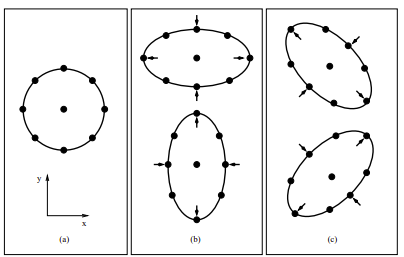
\includegraphics[width=3in]{images_/stretch.png}
    \caption{Effect of the two polarizations of a gravitational wave propagating through a ring of test particles. Source: \citep{doi:10.1142/9789813141766_0001} }
    \label{fig: stretch}
\end{figure}
A ring of particles at rest on the xy-plane in an initial wave-free region of space-time encounters a gravitational wave traveling in the $z$ direction. The arrival of the wave alters the proper separation between the particles. The \textit{plus} polarization of the wave stretches and squeezes the ring along the x- and y-axes, oscillating between the shapes seen in panel (b) of figure \ref{fig: stretch}.\\
Once we understand the effects of a gravitational wave passing on a pair of test particles, we could develop tools to detect that effect, which could involve a laser and an interferometer of arm's length L. Assuming that the gravitational wave's wavelength is substantially larger than the interferometer's size, the equation integration becomes simpler equation \ref{eq: stretch}
\begin{equation}
    \delta x = \frac{h_{xx}}{2}x, \hspace{0.5cm} \delta y = \frac{h_{yy}}{2}y.
\end{equation}
When a gravitational wave passes along the z-direction with polarization $h_{xx} = -h_{yy} = h_{+}(t)$, the change in proper distance and the phase difference between the two beams at the origin are
\begin{equation}
    \frac{\delta L(t)}{L} = h_{+}(t), \hspace{0.8cm} \Delta \phi = 2\pi \frac{L}{\lambda}h_{+}(t)
\end{equation}
The difference in phase between the beams recombining at the beam splitter is proportional to
\begin{equation}
    h(t) \propto \delta (\Delta \phi) \equiv F_{+}h_{+}(t) + F_{\times}h_{\times}(t),
\end{equation}
where $F_{+}$ and $F_{\times}$ are the antenna patterns of the detector. The quantity $h$ is the \emph{gravitational wave strain}.\\
The spatial variation of the gravitational wave in the arms of the interferometer is considered to be insignificant in this derivation. We do not account for the temporal fluctuation of $h(t)$ during the brief interval $\approx 2L$ that the light takes to go back and forth to the mirror. 


\section{Gravitational Waves Of Binary Stars}
Compact objects like neutron stars or black holes that are orbiting each other and are bound together by gravity go through a process called coalescence in which some of their energy is released as gravitational radiation \citep{Blanchet_2002}\citep{coalesence}\citep{thesis}. In gravitational-wave astronomy, these merging binaries are particularly important because they are promising candidates for first detection.

The gravitational wave emanating from pairs of black holes or neutron stars can be described using various analytical and numerical theoretical approaches. During the inspiral phase, the binary's orbital frequency increases as they lose energy to gravitational waves, which can be described by the post-Newtonian approximation. The emitted gravitational wave strain \( h(t) \) \citep{Blanchet_2002}\citep{Hughes_2009} is given by:

\begin{equation}
h(t) = \frac{4G\mu}{c^2R} \left( \frac{G\mathcal{M}}{c^3} \right)^{5/3} f(t)^{2/3} \cos[\phi(t)]
\end{equation}

where:
\begin{itemize}
    \item \( G \) is the gravitational constant,
    \item \( \mu \) is the reduced mass of the binary system,
    \item \( c \) is the speed of light,
    \item \( R \) is the distance to the binary system,
    \item \( \mathcal{M} = (\mu)^{3/5}M^{2/5} \) is the chirp mass, with \( M \) being the total mass,
    \item \( f(t) \) is the gravitational wave frequency,
    \item \( \phi(t) \) is the phase of the wave.
\end{itemize}

The frequency evolution of the gravitational wave, \( f(t) \), as the binary inspirals, can be described by:

\begin{equation}
f(t) = \frac{1}{\pi} \left( \frac{5}{256} \frac{1}{\tau(t)} \right)^{3/8} \left( \frac{c^3}{G\mathcal{M}} \right)^{5/8}
\end{equation}

where \( \tau(t) \) is the time to coalescence.

As the binary reaches the merger phase, numerical relativity simulations are employed to solve the full Einstein field equations, providing accurate descriptions of the gravitational waveforms during the merger and ringdown phases. The merger phase generates a strong gravitational wave signal as the two compact objects collide, forming a single, more massive object.

The ringdown phase follows, where the newly formed object emits gravitational waves as it settles into a stable state. This phase can be described using the quasi-normal modes of the remnant object, typically modeled as a damped sinusoidal wave:

\begin{equation}
h(t) = A e^{-t/\tau} \cos(2\pi f_{\text{ring}} t + \phi)
\end{equation}

where:
\begin{itemize}
    \item \( A \) is the amplitude,
    \item \( \tau \) is the damping time,
    \item \( f_{\text{ring}} \) is the ringdown frequency,
    \item \( \phi \) is the phase.
\end{itemize}

These equations and theoretical models are critical for predicting the gravitational wave signals from coalescing binaries, enabling their detection and analysis in gravitational-wave astronomy \citep{Blanchet_2002}.
